
\title{Thermal building system}
% Use \titlerunning{Short Title} for an abbreviated version of your contribution title if the original one is too long
\author{Roel De Coninck and Lieve Helsen}
\authorrunning{R. De Coninck, L. Helsen}

\maketitle

\abstract{A dynamic thermal system model is developed in Modelica for integrated energy simulation.}

\section{Introduction}

The library is based on Modelica.Thermal.FluidHeatFlow and not on Modelica.Fluid or Modelica.Media.  This makes the library easier to compile by a variety of tools that might not (yet) fully support the  Modelica.Fluid and Modelica.Media libraries.

\section{Hydraulic components}

\subsection{Basic components for Joe the plumber}

\begin{enumerate}
	\item pipe
	\item pump
	\item ambient
	\item three-way valve
	\item pressure grounding
\end{enumerate}

\subsection{Thermal energy storage tank}

\subsubsection{Buffer tank}

\emph{IDEAS.Thermal.Components.Storage.StorageTank}

Buffer tank (no internal heat exhcangers) composed of an array of interconnected pipes with ambient heat losses (= layers).  The number of layers $nbrNodes$ is a parameter and an array of $nbrNodes + 1$ \emph{FlowPort} connectors is available to connect to each intersection between the layers. 

\begin{equation}
mc_p \frac{dT_i}{dt}=\dot{m}_ic_p(T_{i-1} - T_i) + \dot{q}_i
\label{eq:}
\end{equation}

In this equation, $\dot{q}_i$ is composed of different heat transfer phenomena:

\begin{equation}
\dot{q}_i = \dot{q}_{conduction,~i-1} - \dot{q}_{conduction,~i} + \dot{q}_{loss,~i} +  \dot{q}_{buoyancy,~i}
\label{eq:}
\end{equation}

\begin{equation}
\dot{q}_{conduction,~i} = \frac{\lambda_{water} S}{h_{node}} (T_{i-1} - T_i) 
\label{eq:}
\end{equation}

\begin{equation}
\dot{q}_{loss,~i} = UA_{loss}(T_{i} - T_{ambient}) 
\label{eq:}
\end{equation}

\begin{equation}
\dot{q}_{buoyancy,~i} = \text{ if } (T_{i-1} \geq T_i \geq T_{i+1}) \text{ then } 0 \text{ else } ???
\label{eq:}
\end{equation}

A first attempt was to suppose that buoyancy can be modelled with an equivalent thermal conductivity. 

\begin{equation}
\text{ if } (T_{i} \leq T_{i+1}) \text{ then } \dot{q}_{buoyancy} = \lambda_{buoyancy} S (T_{i+1}-T_i)
\label{eq:}
\end{equation}

\begin{figure}%
\begin{left}
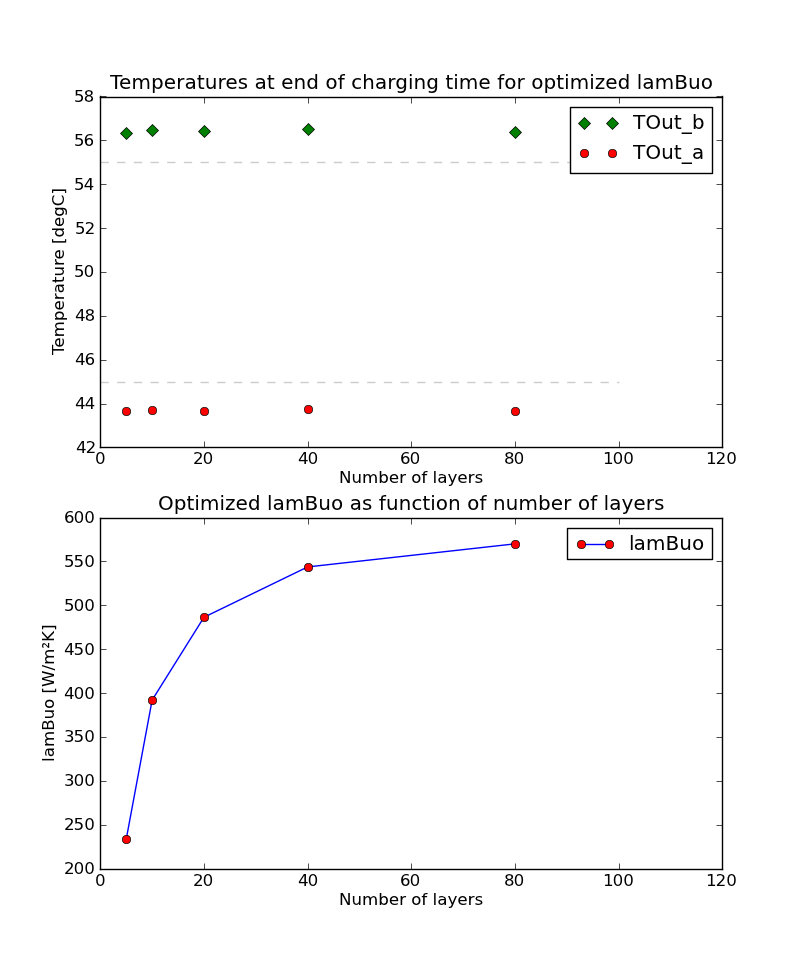
\includegraphics[width=\columnwidth]{Thermal/images/Validation_Vitocell100V390l_ChargingTimeEndTemperatures_Linear.png}% of \columnwidth
\caption{Result of the linear parameter fitting}%
\label{tankinternal}%	
\end{left}
\end{figure}

To find $\lambda_{buoyancy}$, an optimization is carried out in which for different number of nodes, the $\lambda_{buoyancy}$ that assures the best fit of the end temperatures for both charging experiments is found.

The results show that for a given number of nodes, this leads to acceptable validation results for the charging experiment.  However, the equivalent thermal conductivity is strongly dependent on the number of nodes.  As this can be due to the variable node height, mass and DT between the nodes, a model with a parameter that clearly depends on the number of nodes is not useful for sensitivity studies in which for example the tank volume and geometry is changed.

A second approach is to suppose that buoyancy is actually a mass flow rate phenomena, caused by different densities of the water as a function of temperature.  Therefore, the following equation is used as a starting point.

\begin{equation}
\text{ if } (T_{i} \leq T_{i+1}) \text{ then } \dot{q}_{buoyancy} = \dot{m}_{buo} c_p (T_{i+1}-T_i)
\label{eq:}
\end{equation}

We suppose $\dot{m}_{buo}$ depends on the temperature gradient, and is zero when the temperature difference between the layers is zero.

\begin{equation}
\dot{m}_{buo} = k_{buo} {(\frac{dT}{dh}})^{\text{exp}_{buo}}
\label{eq:}
\end{equation}

Again, optimization is used in order to identify $k_{buo}$ and $\text{exp}_{buo}$ as a function of the number of nodes. Again, we see that these coefficients are depending on the number of nodes.  We also see that the sensitivities on the obtained end temperatures in the charging experiment is large.

\begin{figure}%
\begin{left}
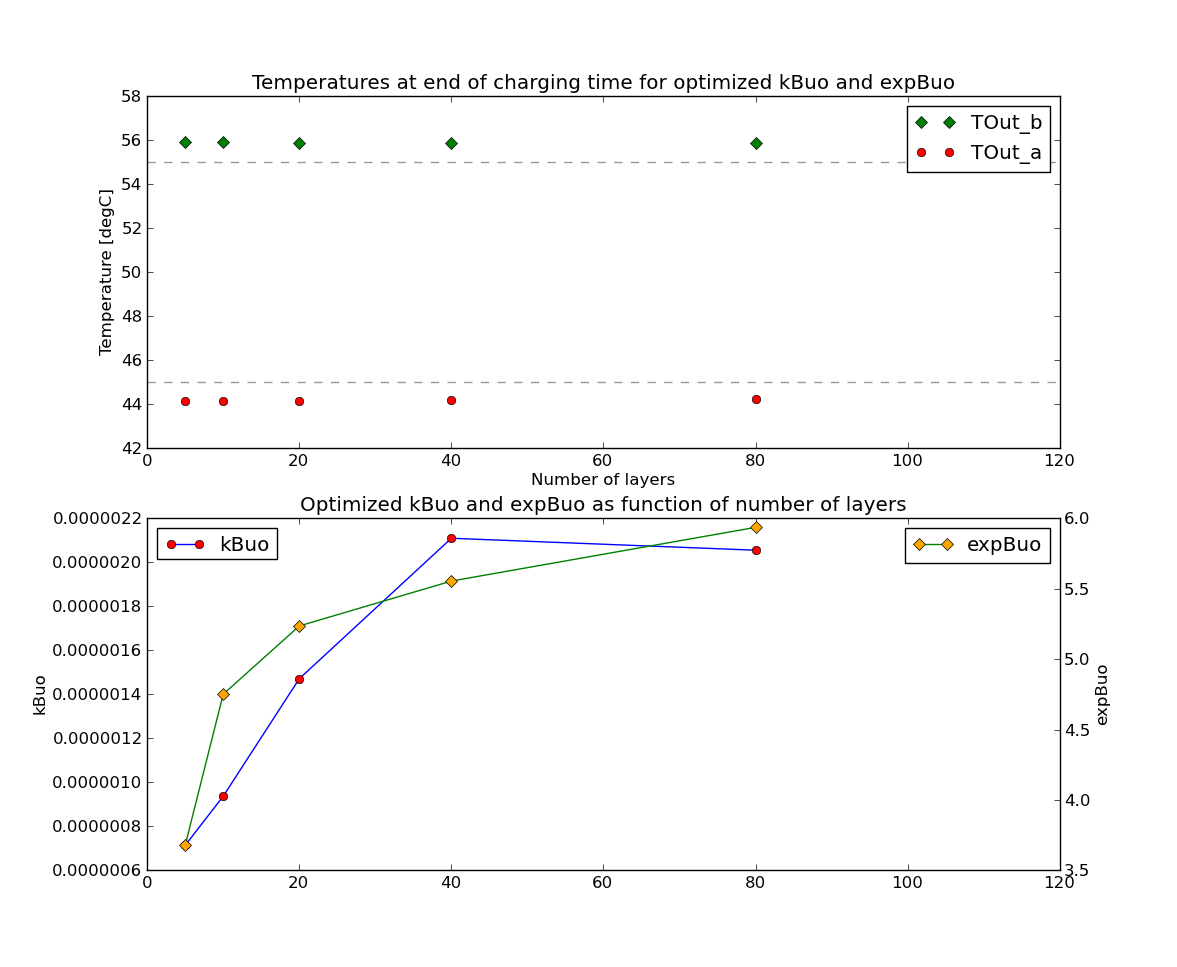
\includegraphics[width=\columnwidth]{Thermal/images/Validation_Vitocell100V390l_ChargingTimeEndTemperatures_NonLinear.png}% of \columnwidth
\caption{Result of the non-linear parameter fitting}%
\label{tankinternal}%	
\end{left}
\end{figure}

\begin{figure}%
\begin{left}
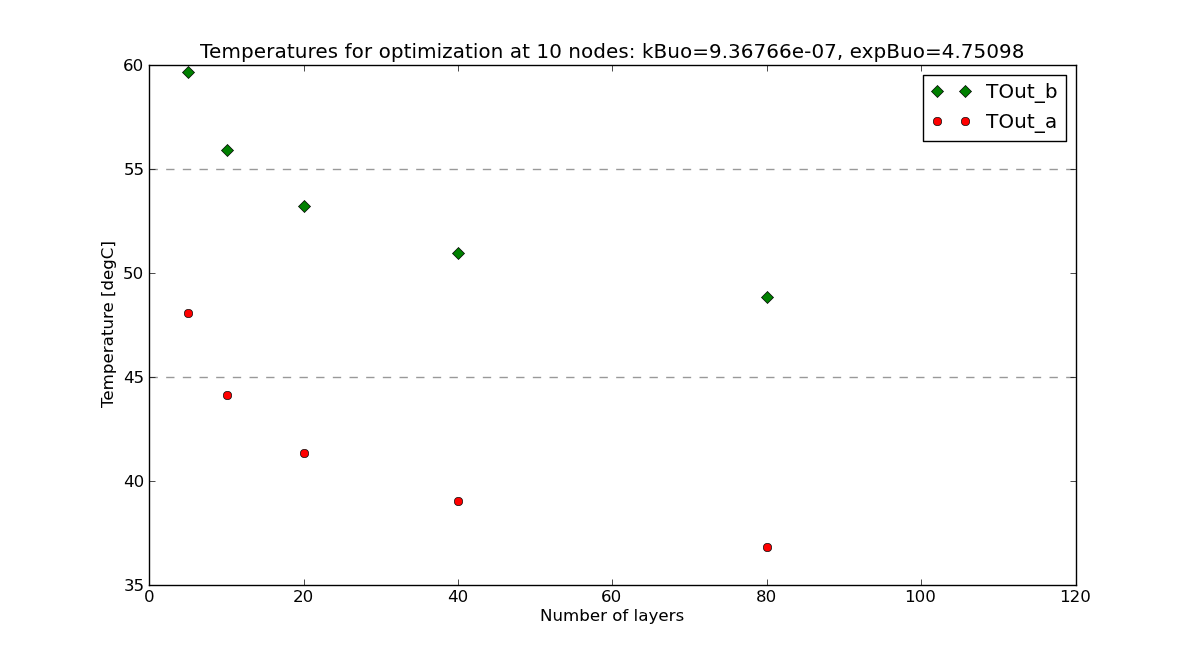
\includegraphics[width=\columnwidth]{Thermal/images/Validation_Vitocell100V390l_ChargingTimeEndTemperatures_nonlin_10nodes.png}% of \columnwidth
\caption{Resulting temperatures when the found values for 10 nodes are used}%
\label{tankinternal}%	
\end{left}
\end{figure}

\subsubsection{Tank with internal heat exchanger}

\emph{IDEAS.Thermal.Components.Storage.StorageTank_OneIntHX}

\vspace{6mm}

This tank is similar to \emph{IDEAS.Thermal.Components.Storage.StorageTank} except that an internal heat exchanger is added.  The heat exchanger can be positioned in any continuous section of layers, it is modelled with one heat exhanger node per tank layer. 

\begin{figure}%
\begin{left}
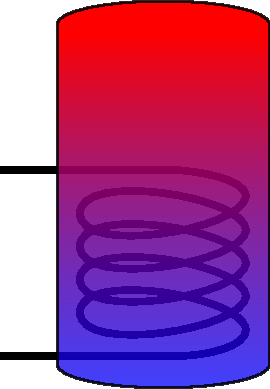
\includegraphics[width=3cm]{Thermal/images/HydraulicScheme.pdf}% of \columnwidth
\caption{Tank with internal heat exchanger}%
\label{tankinternal}%	
\end{left}
\end{figure}

Add heat transfer coefficients and other details.

\subsection{Heat production}

\subsubsection{Partial heater}

\emph{IDEAS.Thermal.Components.Production.Auxiliaries.PartialDynamicHeaterWithLosses}

\vspace{6mm}

All hydraulic heater models extend from this partial heater model.  
tbc

\subsubsection{Boiler}

\subsubsection{Heat pumps}

\begin{enumerate}
	\item modulating air-source hp
	\item ground-source hp
\end{enumerate}

\subsection{Heat emission}

\subsubsection{Partial heat emission model}

\emph{IDEAS.Thermal.Components.Emission.Auxiliaries.Partial_Emission}
\vspace{6mm}

\subsubsection{Radiator}

\subsubsection{Embedded pipe for thermally activated building systems (TABS)}

From ~\cite{Koschenz2000}

\section{Heating systems}

\subsection{Ideal heating}

\subsection{Hydraulic heating}

Main hydraulic scheme with replaceable models for heat production, heat emission, solar thermal system and control.

\subsection{Solar thermal system}

\subsection{Domestic hot water production}

\section{Vertical ground heat exchanger}

\subsection{Model Harm Leenders}

\subsection{Model Dieter Patteeuw}

\section{Control}


%\bibliography{Thermal/MyBibTexLibrary}









